\section{Experimentos computacionales}
\label{sec:experimentos}

\subsection{Diseño experimental}
\textbf{Máquina:} Apple M1; \textbf{solver:} Gurobi 12.0.0; backend único Gurobi.
\textbf{Configuración:} algoritmo de dos fases, warm-start activo por defecto (\texttt{--coldstart}
para el comparativo), \texttt{MIPGap}$=10^{-10}$, sin límite de tiempo interno del solver (todas
las instancias reportadas cierran a optimalidad). \textbf{Sin} PopStar: el paper usa esa
heurística primal externa para obtener buenas cotas superiores de Fase 1; este repositorio usa un
redondeo propio más simple. \textbf{Sin} \emph{reduced-cost fixing} ni \emph{constraint reduction}.
Todos los números provienen de
\texttt{results/} (CSV y \texttt{logs/}); cada corrida deja un log con prueba de callback. Para
la versión final se conserva además un snapshot curado en \texttt{results/curated/}, validado por
\texttt{scripts/validate\_results.py}, porque \texttt{results/benchmark.csv} es append-only y puede
contaminarse con reruns.

Se reportan cinco bloques: (i) corrección y desempeño en OR-Library; (ii) comparación contra el
paper en \texttt{rl1304}; (iii) baseline F1 (monolithic model) parcial; (iv) grilla sintética de estrés;
(v) efecto del warm-start. Cuatro figuras agregan el comportamiento.
El pipeline de interacción para preparar/correr el catálogo local está expuesto por
\texttt{scripts/paperbench.py}. El comando completo usado para el snapshot final fue:
\begin{lstlisting}[language=bash,numbers=none]
.venv/bin/python scripts/paperbench.py run --set current --timeout 300 \
  --out results/curated/paperbench_current.csv \
  --log-dir results/logs/paperbench_current
.venv/bin/python scripts/paperbench.py summarize --csv results/curated/paperbench_current.csv
.venv/bin/python scripts/paperbench.py validate --csv results/curated/paperbench_current.csv
\end{lstlisting}
La salida esperada del resumen es: 26 filas OK, 25/25 óptimos conocidos coincidentes; el caso
restante es \texttt{kroA100}, sin óptimo oficial/paper cargado en el catálogo.

\subsection{Caso base y corrección en OR-Library}
Las 15 instancias \texttt{pmed} cierran al \textbf{óptimo oficial} con brecha $0\%$ (delta$=0$).
Fuente: \texttt{results/curated/orlib\_optima\_check.csv}.

\begin{table}[h]\centering\small
\begin{tabular}{lrrrrrrrr}
\toprule
inst. & $N$ & $p$ & $LB_1$ & $UB_1$ & óptimo & oficial & iter & nodos \\
\midrule
pmed1  & 100 & 5   & 5819.0 & 5819.0 & 5819 & 5819 & 6 & 1 \\
pmed2  & 100 & 10  & 4088.5 & 4116.0 & 4093 & 4093 & 6 & 1 \\
pmed3  & 100 & 10  & 4240.5 & 4250.0 & 4250 & 4250 & 6 & 3 \\
pmed4  & 100 & 20  & 3034.0 & 3034.0 & 3034 & 3034 & 5 & 1 \\
pmed5  & 100 & 33  & 1355.0 & 1355.0 & 1355 & 1355 & 5 & 1 \\
pmed6  & 200 & 5   & 7783.5 & 7867.0 & 7824 & 7824 & 6 & 7 \\
pmed7  & 200 & 10  & 5631.0 & 5631.0 & 5631 & 5631 & 6 & 1 \\
pmed8  & 200 & 20  & 4445.0 & 4445.0 & 4445 & 4445 & 5 & 1 \\
pmed9  & 200 & 40  & 2734.0 & 2734.0 & 2734 & 2734 & 6 & 1 \\
pmed10 & 200 & 67  & 1255.0 & 1255.0 & 1255 & 1255 & 9 & 1 \\
pmed11 & 300 & 5   & 7693.3 & 7696.0 & 7696 & 7696 & 9 & 1 \\
pmed12 & 300 & 10  & 6625.8 & 6638.0 & 6634 & 6634 & 7 & 7 \\
pmed13 & 300 & 30  & 4374.0 & 4374.0 & 4374 & 4374 & 5 & 1 \\
pmed14 & 300 & 60  & 2967.2 & 2971.0 & 2968 & 2968 & 8 & 1 \\
pmed15 & 300 & 100 & 1729.0 & 1729.0 & 1729 & 1729 & 7 & 1 \\
\bottomrule
\end{tabular}
\caption{OR-Library: 15/15 al óptimo oficial, delta$=0$. ``iter''$=$separaciones de Fase 1;
``nodos''$=$nodos de B\&B en Fase 2. Todo el conjunto se resuelve en $<0.36$\,s
(snapshot curado: \texttt{results/curated/benchmark\_current.csv}).}
\label{tab:orlib}
\end{table}

\textbf{Lectura.} En la mayoría de las instancias $LB_1=UB_1=$ óptimo: la Fase 1 ya cierra el
problema y la Fase 2 confirma en $1$ nodo. Solo \texttt{pmed3}, \texttt{pmed6} y \texttt{pmed12}
requieren ramificar ($3$, $7$, $7$ nodos), justo donde $UB_1>$ óptimo.

\subsection{Extensión OR-Library \texttt{pmed1}--\texttt{pmed40}}
Además del bloque principal \texttt{pmed1}--\texttt{pmed15}, la evidencia consolidada contiene
\texttt{pmed16} como smoke verificado y \texttt{pmed17}--\texttt{pmed40} como extensión local. No
fue una única campaña global: son corridas controladas y trazadas en CSV/logs distintos, todas
bajo timeout externo de 300 segundos.

\begin{table}[h]\centering\small
\begin{tabular}{lrrl}
\toprule
grupo & filas & resultado & evidencia \\
\midrule
\texttt{pmed1}--\texttt{pmed15} & 15 & 15/15 \texttt{OPT\_MATCH} & \texttt{benders\_300s\_campaign.csv} \\
\texttt{pmed16} & 1 & \texttt{OPT\_MATCH}, obj. 8162 & \texttt{orlib\_pmed16\_smoke\_300s.csv} \\
\texttt{pmed17}--\texttt{pmed40} & 24 & 24/24 \texttt{OPT\_MATCH} & \texttt{orlib\_pmed17\_pmed40\_300s.csv} \\
\midrule
total consolidado & 40 & 40/40 óptimos oficiales & \texttt{report/REPORT\_TABLES.md} \\
\bottomrule
\end{tabular}
\caption{OR-Library consolidado. \texttt{pmed17}--\texttt{pmed40} tiene 0 timeouts y máximo
$T_{tot}=10.695018$s en \texttt{pmed36}.}
\label{tab:orlib40}
\end{table}

\subsection{Comparación contra el paper (\texttt{rl1304})}
Sobre las mismas instancias TSPLIB \texttt{rl1304} de la Tabla 2 de Duran-Mateluna, Ales \&
Elloumi (2023) se comparan los óptimos y cotas. Los valores del paper fueron transcritos en
\texttt{scripts/compare\_paper.py}; el CSV resultante es
\texttt{results/curated/comparison\_vs\_paper.csv}.

\begin{table}[h]\centering\small
\begin{tabular}{rrrrrrrr}
\toprule
$p$ & óptimo paper & óptimo nuestro & $\Delta$ & $LB_1$ paper & $LB_1$ nuestro & $UB_1$ paper & $UB_1$ nuestro \\
\midrule
5   & 3099073 & 3099073 & 0 & 3099073 & 3099073 & 3099073 & 3099073 \\
10  & 2134295 & 2134295 & 0 & 2131788 & 2131788 & 2134295 & 2243679 \\
20  & 1412108 & 1412108 & 0 & 1412108 & 1412108 & 1412108 & 1412108 \\
50  &  795012 &  795012 & 0 &  795012 &  795012 &  795012 &  795012 \\
100 &  491639 &  491639 & 0 &  491507 &  491506 &  491788 &  496403 \\
200 &  268573 &  268573 & 0 &  268573 &  268573 &  268573 &  268573 \\
300 &  177326 &  177326 & 0 &  177318 &  177318 &  177339 &  179952 \\
400 &  128332 &  128332 & 0 &  128332 &  128332 &  128332 &  128332 \\
500 &   97024 &   97024 & 0 &   97018 &   97018 &   97034 &   97034 \\
\bottomrule
\end{tabular}
\caption{\texttt{rl1304}: \textbf{9/9 óptimos coinciden} ($\Delta=0$). El $LB_1$ de Fase 1
coincide con el del paper (a $\pm1$). El $UB_1$ a veces es peor que el del paper porque no usamos
PopStar (ver Sección~\ref{sec:resultados}). Tiempos no comparados directamente
(máquinas/solvers distintos: paper XEON\,W-2145/CPLEX\,20.1; nosotros M1/Gurobi\,12).}
\label{tab:paper}
\end{table}

\subsection{Baseline F1 (monolithic model) parcial}
La pauta del curso pide una implementación base. Aquí \emph{monolithic} significa cargar la
formulación estándar completa directamente al solver, sin Benders ni lazy constraints. Se
implementó y ejecutó F1 de esa forma solo en cinco instancias pequeñas/medianas; esto
\textbf{no} es un benchmark completo de F1--F4. Evidencia:
\texttt{report/evidence/csv/monolithic\_f1\_300s.csv}.

\begin{table}[h]\centering\small
\begin{tabular}{lrrrrrr}
\toprule
instancia & $N$ & $p$ & F1 obj. & F1 runtime & Benders $T_{tot}$ & nota \\
\midrule
\texttt{toy1} & 4 & 2 & 6 & 0.024817 & 0.040586 & F1 más rápido \\
\texttt{pmed1} & 100 & 5 & 5819 & 0.436110 & 0.035466 & Benders más rápido \\
\texttt{pmed2} & 100 & 10 & 4093 & 0.441374 & 0.083832 & Benders más rápido \\
\texttt{pmed6} & 200 & 5 & 7824 & 6.991906 & 0.310273 & Benders más rápido \\
\texttt{kroA100} & 100 & 10 & 30539 & 0.461514 & 0.067967 & Benders más rápido \\
\bottomrule
\end{tabular}
\caption{Baseline F1 parcial: cinco filas, 0 timeouts. La comparación solo vale en este solape;
no se implementaron F2/F3/F4 como monolithic models en una campaña completa.}
\label{tab:f1baseline}
\end{table}

\subsection{Grilla sintética de estrés local}
Se generaron 18 instancias euclidianas determinísticas con seed \texttt{20260622},
$N\in\{100,250,500,1000,2000,5000\}$ y $p$ igual a 5\%, 10\% y 20\% de $N$. Todas terminaron bajo
timeout externo de 300 segundos. Todas tienen estado \texttt{OPTIMAL\_NO\_KNOWN}: el solver
certifica optimalidad interna, pero no hay óptimo externo/paper contra el cual comparar.

\begin{table}[h]\centering\small
\begin{tabular}{rrrr}
\toprule
$N$ & $p=5\%$ $T_{tot}$/nodos/cuts & $p=10\%$ $T_{tot}$/nodos/cuts & $p=20\%$ $T_{tot}$/nodos/cuts \\
\midrule
100 & 0.484661 / 1 / 93 & 0.037117 / 1 / 115 & 0.030035 / 1 / 88 \\
500 & 0.710534 / 59 / 721 & 0.141580 / 1 / 649 & 0.330849 / 1 / 516 \\
1000 & 3.151895 / 7 / 1385 & 0.591020 / 1 / 1226 & 0.695118 / 3 / 1008 \\
2000 & 3.043141 / 1 / 2725 & 2.442365 / 15 / 2494 & 1.649372 / 1 / 2023 \\
5000 & 44.247668 / 292 / 6874 & 7.709930 / 8 / 6049 & 7.055344 / 6 / 4870 \\
\bottomrule
\end{tabular}
\caption{Estrés sintético local hasta $N=5000$: 18/18 filas sin timeout. No es campaña del paper y
no tiene óptimos externos conocidos. Fuente: \texttt{synthetic\_stress\_300s.csv}.}
\label{tab:synthetic}
\end{table}

\subsection{Efecto del warm-start}
Heredar el pool de cortes de Fase 1 reduce drásticamente el árbol de B\&B. Fuente:
\texttt{results/curated/warmstart\_comparison.csv}.

\begin{table}[h]\centering\small
\begin{tabular}{lrr rr rr}
\toprule
 & \multicolumn{2}{c}{nodos B\&B} & \multicolumn{2}{c}{lazy constraints} & \multicolumn{2}{c}{$T_2$ [s]} \\
inst. ($p=5$) & cold & warm & cold & warm & cold & warm \\
\midrule
pmed1  & 223 & \textbf{1} & 513  & 90  & 0.047 & 0.016 \\
pmed6  & 632 & \textbf{7} & 1053 & 240 & 0.143 & 0.600 \\
pmed11 & 352 & \textbf{1} & 1768 & 308 & 0.030 & 0.940 \\
\bottomrule
\end{tabular}
\caption{Warm-start vs cold-start. Los nodos y las lazy constraints caen fuertemente. El wall-time es
\emph{mixto} en estas instancias sub-segundo: la precarga de cientos de cortes (337/694/1285) a
veces cuesta más de lo que ahorra. Beneficio en nodos $\ne$ beneficio en tiempo a esta escala.}
\label{tab:warm}
\end{table}

\subsection{Prueba de que es branch-and-Benders-cut real}
Cada corrida \texttt{--mode full} registra la actividad del callback. Por ejemplo
(\texttt{results/logs/pmed1.pmp\_p5\_full.log}): \texttt{separation\_calls=3}, \texttt{lazy\_cuts=90},
\texttt{bb\_nodes=1}, \texttt{is\_branch\_and\_benders\_cut=YES}. En \texttt{rl1304} $p=5$:
\texttt{lazy\_cuts=1850}. Tener \texttt{lazy\_cuts}>0 confirma que la Fase 2 \emph{no} degenera a
un B\&B ordinario: el callback está agregando cortes de Benders durante el árbol.

\subsection{Figuras agregadas}
Las cuatro figuras (generadas solo de CSV reales por \texttt{scripts/plot\_results.py}) son:
\begin{figure}[h]\centering
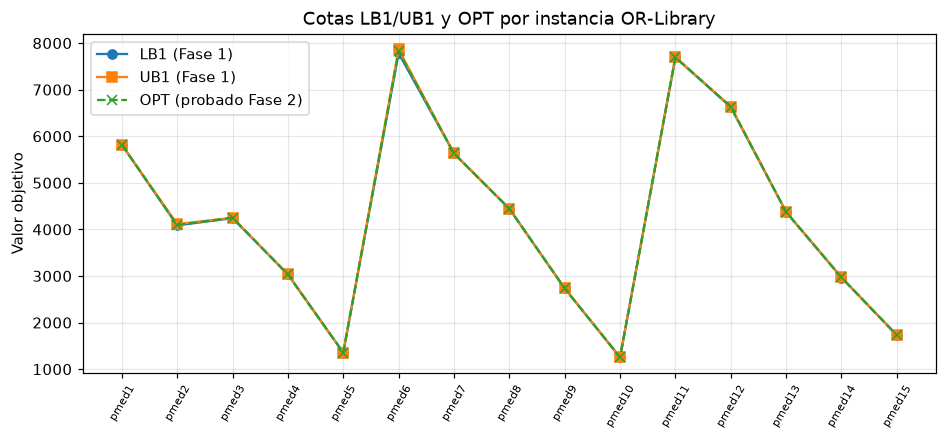
\includegraphics[width=0.48\textwidth]{figures/plot_a_bounds_orlib.png}\hfill
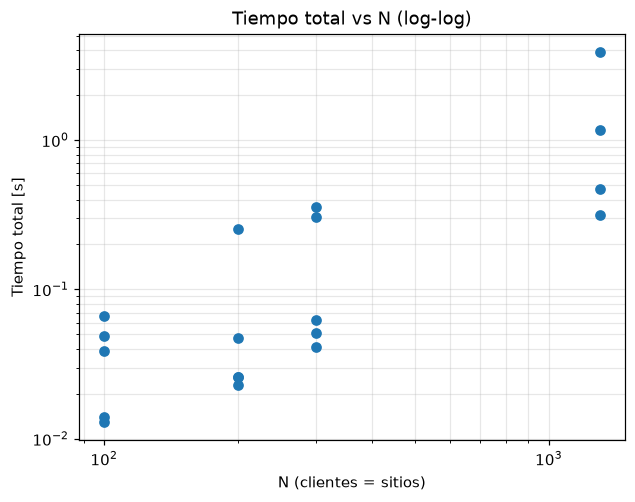
\includegraphics[width=0.48\textwidth]{figures/plot_b_time_vs_N.png}
\caption{(izq.) $LB_1$, $UB_1$ y óptimo por instancia OR-Library. (der.) Tiempo total vs $N$ (log-log).
Fuente: \texttt{results/curated/orlib\_optima\_check.csv} y \texttt{results/curated/benchmark\_current.csv}.}
\end{figure}
\begin{figure}[h]\centering
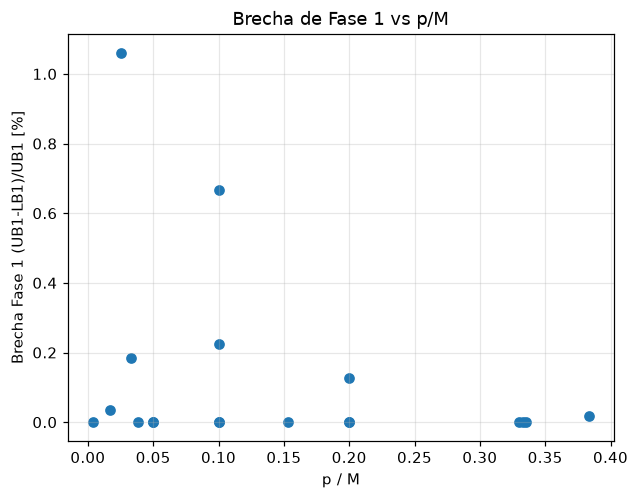
\includegraphics[width=0.48\textwidth]{figures/plot_c_gap_vs_pM.png}\hfill
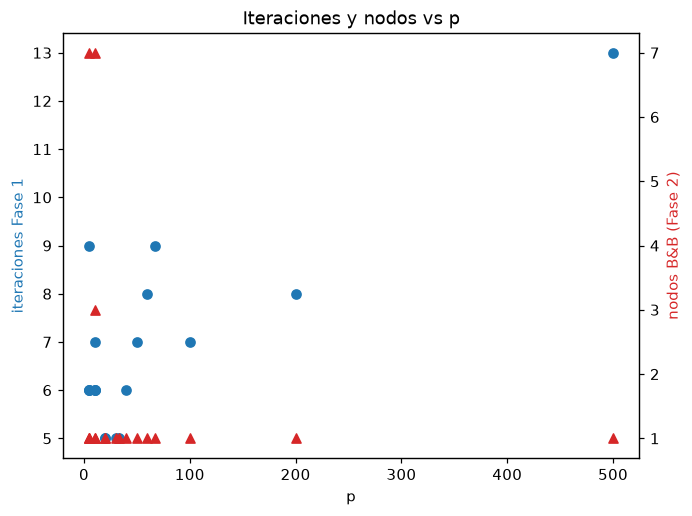
\includegraphics[width=0.48\textwidth]{figures/plot_d_iter_nodes_vs_p.png}
\caption{(izq.) Brecha de Fase 1 $(UB_1-LB_1)/UB_1$ vs $p/M$. (der.) Iteraciones (Fase 1) y nodos
(Fase 2) vs $p$. Fuente: \texttt{results/curated/benchmark\_current.csv}.}
\end{figure}
